\section{Methodology}\label{sec:meto}
% Conceptual explanation of implementation, configuration, and setup. (May use code snippets and
% screenshots to explain concepts, but not full code listings.)
After deciding on our project topic we fixed our software requirements in more concrete form. Having done so we identified that it would be most beneficial to divide our future code into front end and backed with the main interface being between graphical user interface (GUI) and text data structure. The \verb|textStructure.h| header is the main interface connecting the GUI in \verb|main.c| and the actual text data structure implementation in \verb|textStructure.c| \cite{GithubRepo}. The other files are mostly built around these two central pieces of code. A more visual layout can be seen in \ref{fig:codeStruct}.
\begin{figure}[H]
\caption{Project Code Structure}
\noindent\begin{tikzpicture}[ 
    % Define node styles
    scale = 1,
    node distance = 0.5cm,
    minimum height = 1cm,
    imp/.style={rectangle, rounded corners, fill=teal!65, draw, align=center},
    file/.style={rectangle, rounded corners, fill=teal!25, draw, align=center},
    adj/.style={rectangle, rounded corners, fill=gray!10, draw, align=center},
    division1/.style={rectangle, fill=teal!5, draw=teal!20, line width=1pt, inner sep=5mm},
    division2/.style={rectangle, fill=teal!5, draw=teal!20, line width=1pt, inner sep=5mm},
    division3/.style={rectangle, fill=gray!5, draw=gray!50, line width=1pt, inner sep=5mm},
]

% Main nodes
\node[file] (guiUt) {guiUtilities};
\node[file, right= 1.5of guiUt] (fileM) {fileManager};
\node[file, right= of fileM] (undo) {undoRedoUtilities};
\node[file, right= of undo] (stats) {statistics};

\node[imp, above= of guiUt] (main) {main};
\node[imp, above= of undo] (txtStruct) {textStructure};

\node[adj, right = 1.5of stats] (profiler){profiler};
\node[adj, above= of profiler] (debug) {debugUtil};

% Background division boxes using fit library
\begin{scope}[on background layer]
    \node[division1, fit=(main)(guiUt)] (division1) {};
    \node[above= 0.1of division1] {\bfseries Front End};
    \node[division2, fit=(txtStruct)(fileM)(undo)(stats)] (division2) {};
    \node[above= 0.1of division2] {\bfseries Back End};
    
    \node[division3, fit=(profiler)(debug)] (division3) {};
    \node[above= 0.1of division3] {\bfseries debugging \& analysis};
\end{scope}

% Arrows for main flow
\draw[latex-latex,  line width=2pt] (main) -- (txtStruct);

\draw[latex-latex,  line width=0.5pt] (main) -- (guiUt);
\draw[latex-latex,  line width=0.5pt] (main) -- (fileM);
\draw[latex-latex,  line width=0.5pt] (txtStruct) -- (fileM);
\draw[latex-latex,  line width=0.5pt] (txtStruct) -- (undo);
\draw[latex-latex,  line width=0.5pt] (txtStruct) -- (stats);

\end{tikzpicture}
\label{fig:codeStruct}
\end{figure}

\begin{figure}[H]
\caption{High level text data structure (sequence) illustration}
\centering
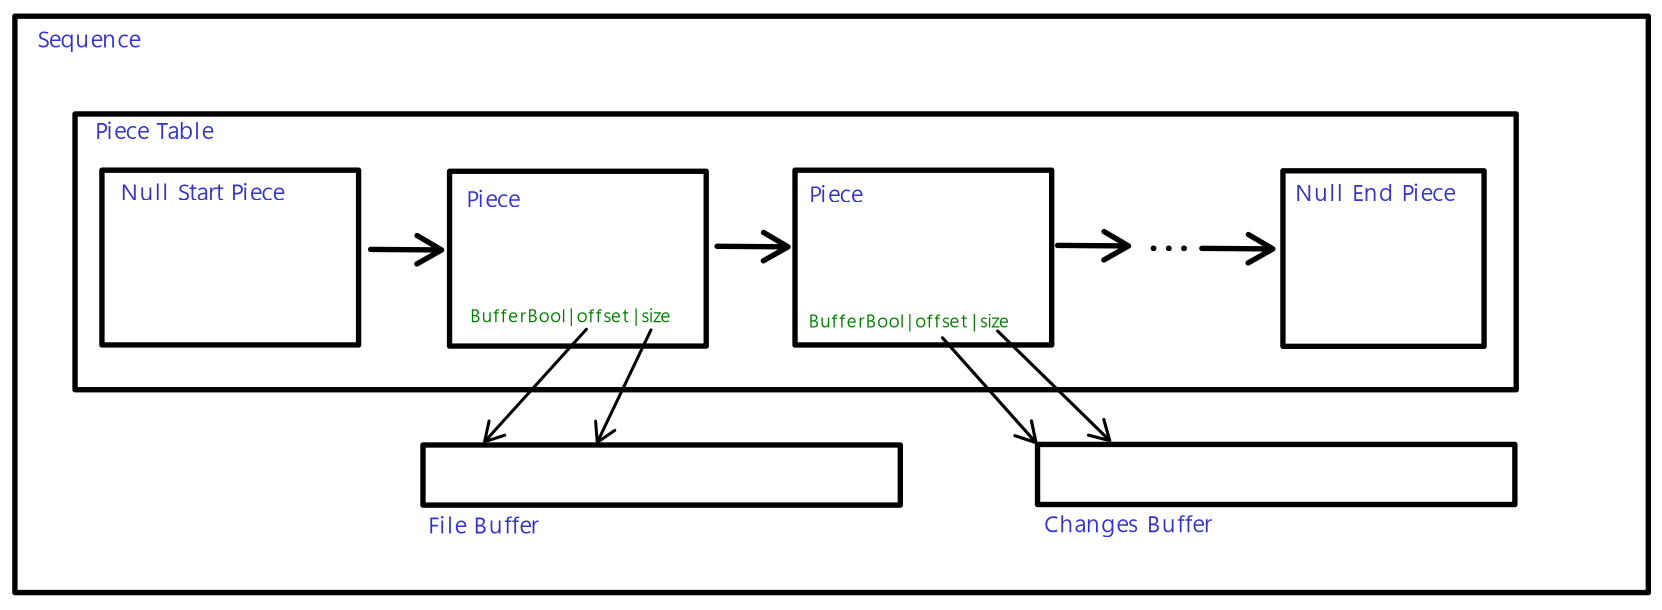
\includegraphics[width=0.8\textwidth]{./images/sequenceIllustration.png}
\label{fig:sequence}
\end{figure}

\textbf{File management}(see \verb|fileManager.c| \cite{GithubRepo}) The way we load files into the editor is optimized even for very large files (we tested up to 5.5 GB text files). This partly because we directly map the file buffer of the sequence onto a mmap of the opened file. This directly leverages the speed and adavantage of the Linux mmap capabilites. Uppon save we also use mmaps to write, but we decided to still take the slight overhead of copying the original file to a temporary location in order to keep the sequece's peice table in it's current state and there for also the whole undo history alive. Otherwise it would need to be reset each time a save is done, which we found not very user friendly. %Last but not least we also added a bonus feature that makes a backup before saving to a file, in case the user accidentally overwrote content of the file, and wishes to recover to the state before that last save.

%GUI
\noindent
\\\verb|print_items_after| is one of our most important parts and our method to that displays text in our terminal. Prints a certain number of lines starting from a chosen atomic position in our text sequence.
Checks if sequence exists and line break standards. If good proceeds. It walks through blocks of text data and handles things liek UTF-8 character boundaries, skips control characters and detects line breaks or end-of-block to finish a text line.
\\Changes current line segment to wide-character string for terminal compatibility.
Output is the processed string that goes to the terminal at correct screen position.
\\For efficiency it only prints lines that are actually visible on the terminal, so out of view lines don't get printed. For that we have a variable that has the absolute position of the line at the top of the screen (e.g. top line is actually the 5th line in the entire text).
Also this is where the lineStats get update and if a line goes across multiple blocks the counters(atomicsInLine, nbrOfUtf8CharsNoControlCharsInLine) carry over to next block
\\
\\In \verb|guiUtilities| we have our line statistics like what is the current line number at the top of the screen or how many chars are in the specified line. The methods in here are used for things like scrolling, jumping to a specific line when using the search function or managing the line stats.
Standouts are the converter from UTF-8 to wide characters and a way to translate cursor position to a position in our data structure.
\\
\\Our Cursor refreshs independent of our text. That means when our cursor moves position it doesn't cause the text to also be refreshed, that would be a big performance hit.